\documentclass{article}
\usepackage{amsmath}
\usepackage{amssymb}
\usepackage{gensymb}
\usepackage{float}
\usepackage[top=1in, bottom=1in, left=1in, right=1in]{geometry}
\usepackage{graphicx}
\usepackage{rotating}
\usepackage{multirow}
\usepackage{enumitem}
\usepackage{amsfonts}
\usepackage{bbm}
\usepackage{wrapfig}
\usepackage{array}
\usepackage{float}
\usepackage{caption}
\usepackage{subcaption}
\usepackage{setspace}
\usepackage{ragged2e}
\newcolumntype{K}[1]{>{\centering\arraybackslash}p{#1}}
\usepackage[hidelinks]{hyperref}
\makeatletter
\newcommand*{\rom}[1]{\expandafter\@slowromancap\romannumeral #1@}
\makeatother
\graphicspath{ {Figures/} }
\begin{document}
	
	\everymath{\displaystyle}
	\begin{titlepage}	 	
		\center
		\text{}\\[3cm]
		\linespread{2}\huge \bfseries MP6: Visual Face Detection
		\center\textsc{\Large ECE 417 Fall 2017}\\[1cm]
		\Large\center\textsc{Yuchen Liang\\ Zixu Zhang  }\\[1.4cm]
		\Large \today\\
		\vfill
	\end{titlepage}
	%\tableofcontents\newpage
	\setlength{\baselineskip}{24pt}
	\onehalfspacing
	\section{Introduction}
	In this MP, we use Adaboost algorithm combined with Viola-Jones features to conduct face recognition of  images. We trained 40 iterations of weak classifier use 126 labeled images, and constructed a strong classifier for face detection of the rest 42 images. In this report, we report unweighted error rates of both weak and strong classifiers and also weighted error rate of weak classifiers in each iteration. 
	
	\section{Method}
	\subsection{Adaboost Weak Classifier Training}
	First, we assume that we have $N$ training images, and each of them have $R$ two-class labeled rectangle $Y$. The general Adaboost Algorithm is shown as following. In training, we label rectangle with face as $1$, and non-face rectangle as $0$.
	\begin{enumerate}[label=\arabic*)]
	\item On line 25, we initialize a weight matrix $W$, such that $W\in\mathbb{R}^{N\times R}$, and each elements $w_{ij}=\frac{1}{NR}$. 
	\item At $t$ th iteration, we can find a weak classifier $h_t(\mathbf{X},p,\theta)$, where $\mathbf{X}$ are set of calculated features, $p$ is the polarity, and $\theta$ is threshold. This is complished from line 44 to 50. Classification for $j$ th rectangle in $i$ the image is defined as  
	\begin{equation}
	h_t(i,j)=\bigg\{\begin{array}{cc}
	1,& p{X}_{ij}<p\theta\\
	0,& p{X}_{ij}\geq p\theta
	\end{array}
	\end{equation}
	For $t$ th weak classifier, we can find corresponding weighted classification error $\epsilon_t$
	\begin{equation}
	\epsilon_t=\sum_{i=1}^{N}\sum_{j=1}^{R}w_{ij}\mathbbm{1}_{h_{ij}\neq Y_{ij}}
	\end{equation}
	\begin{equation}
	\beta_t=\frac{\epsilon_t}{1-\epsilon_t}
	\end{equation}
	\item We update our weight matrix $W$ as
	\begin{equation}
	\tilde{w}_{ij}=\bigg\{\begin{array}{cc}
	w_{ij}\beta_t &h_{ij}= Y_{ij}\\
	w_{ij} & h_{ij}\neq Y_{ij}
	\end{array}
	\end{equation}
	Then, we normalize our updated weight matrix as 
	\begin{equation}
	w_{ij}=\frac{\tilde{w}_{ij}}{\sum_{i=1}^N\sum_{j=1}^R\tilde{w}_{ij}}
	\end{equation}

	\justify In this way, we increse the weight of wrong label, but reduce the weight of accurate label to ensure the accuracy improvement over iterations.
\end{enumerate}
	\subsection{Scalar Features}
	\justify In this MP, we use Viola-Jones features for face detection. In each grayscale image $I$, we are able to find its integral image $II$ as 
	\begin{equation}
	II(x,y)=\sum_{i\leq x,j\leq y}I(i,j)
	\end{equation}
	\justify In this way, it is efficient to calculate the sum of features of any rectangle subsection, by linear combination of integral image values of four corners.	For each labeled rectangle in the set $Y$, we have identify its location in image with four parameters $[X_m,Y_m,W,H]$, where $[X_m,Y_m]$ is the pixel coordinate of its upper right corner, and $W$ and $H$ are its width and height. Similarly, we can identify the location of some subrectangle in side as $fr=[f_X,f_Y,f_W,f_H]$, such that the upper right corner of the subrectangle is $[X_m+Wf_X,Y_m+Hf_Y]$. The width and height of subrectangle is $[Wf_W,Hf_H]$.\\
	\begin{figure}[H]
		\vspace{-1em}
		\centering
		\begin{subfigure}{0.14\textwidth}
			\centering
			\includegraphics[height=1in]{o1}
			\caption{q=1}
			\label{o1}
		\end{subfigure}~
		%
		\begin{subfigure}{0.14\textwidth}
			\centering
			\includegraphics[height=1in]{o2}
			\caption{q=2,v=0}
			\label{o2}
		\end{subfigure}~
		%
		\begin{subfigure}{0.14\textwidth}
			\centering
			\includegraphics[height=1in]{o3}
			\caption{q=2,v=1}
			\label{o3}
		\end{subfigure}~
		%
		\begin{subfigure}{0.14\textwidth}
			\centering
			\includegraphics[height=1in]{o4}
			\caption{q=3,v=0}
			\label{o4}
		\end{subfigure}~
		%
		\begin{subfigure}{0.14\textwidth}
			\centering
			\includegraphics[height=1in]{o5}
			\caption{q=3,v=1}
			\label{o5}
		\end{subfigure}~
		%
		\begin{subfigure}{0.14\textwidth}
			\centering
			\includegraphics[height=1in]{o6}
			\caption{q=4}
			\label{o6}
		\end{subfigure}~
	\caption{Six Feature Orders}
	\vspace{-1.5em}
	\end{figure}
	\justify Figure \ref{o2}  is the sum of the right half, minus the sum of the left half. Figure \ref{o3} is the sum of the bottom half, minus the sum of the top half. Figure \ref{o4} is the sum of the outer thirds, minus the sum of the middle third. Figure \ref{o5} is the sum of the outer thirds, minus the sum of the middle third. Figure \ref{o6} is the sum of the main diagonal quadrants, minus the sum of the off-diagonal quadrants. Scalar feature extraction of a given subrectangle is done in function \texttt{rectfeature}.\\
	
	\justify In order to find the optimal subrectangle, we divide each labeled rectangle into $6\times6$ grids and do exhaustic searches to find a combination of subrectangle and feature order with minimum weighted error $\epsilon_t$ that is used in weak classifier training. The exhaustic search are finished in line 29 to 57 in the code. After each iteration, we store the optimal subrectangle $fr_t$, threshold $\theta_t$, polarity $p_t$ and $\beta_t$ of each iteration as trained classifier.
	
	\subsection{Strong Classifier and Testing}
	\justify We first introduce a weight parameter $\alpha_t$ for each iteration $t$, and define it as
	\begin{equation}
	\alpha_t=-\ln\frac{\epsilon_t}{1-\epsilon_t}=-\ln\beta_t
	\end{equation}
	such that $\alpha_t$ is monotonically decreasing function of $\epsilon_t$.\\
	
	\justify In testing, we say that rectangle with face is labeled as $1$, and non-face rectangle is labeled as $-1$. Since we have 40 iterations of training, we obtained 40 optimal subrectangles for classification. First, we use our subrectangles at $t$ th iteration to calculate scalar features of test images on line 77 by \texttt{rectfeature}. With trained threshold $\theta_t$, and polarity $p_t$,  we are able to use weak classifier to obtain the classification $h_t$ of our test images by modified equation 1 as following.
	\begin{equation}
	h_t(i,j)=\bigg\{\begin{array}{cc}
	1,& p{X}_{ij}<p\theta\\
	-1,& p{X}_{ij}\geq p\theta
	\end{array}
	\end{equation}
	After iterating through all trained classifier, we are able to construct a strong classifier $H_t$ as following,
	\begin{equation}
	\tilde{H}_t(i,j)=\sum_{k=1}^{t}\alpha_kh_k(ij)
	\end{equation}
	\begin{equation}
    H_t(i,j)=\bigg\{\begin{array}{c c}
    1 & \tilde{H}_t(i,j)>0\\
    -1 & \tilde{H}_t(i,j)<0
    \end{array}
	\end{equation}
	 Therefore, we can calculated unweighted errors of both strong and weak classifier of testing images as
	 \begin{equation}
	 \epsilon_{weak}=\frac{\sum_{i=1}^N\sum_{j=1}^R\mathbbm{1}_{h_t(i,j)\neq Y_{ij}}}{NR}
	 \end{equation}
	 \begin{equation}
	 \epsilon_{strong}=\frac{\sum_{i=1}^N\sum_{j=1}^R\mathbbm{1}_{H_t(i,j)\neq Y_{ij}}}{NR}
	 \end{equation}
	
	
	
	\section{Result}
	We plotted unweighted errors of both strong and weak classifier and weighted error rates over 40 iterations in Figure \ref{fig:result}
	\begin{figure}[H]
		\centering
		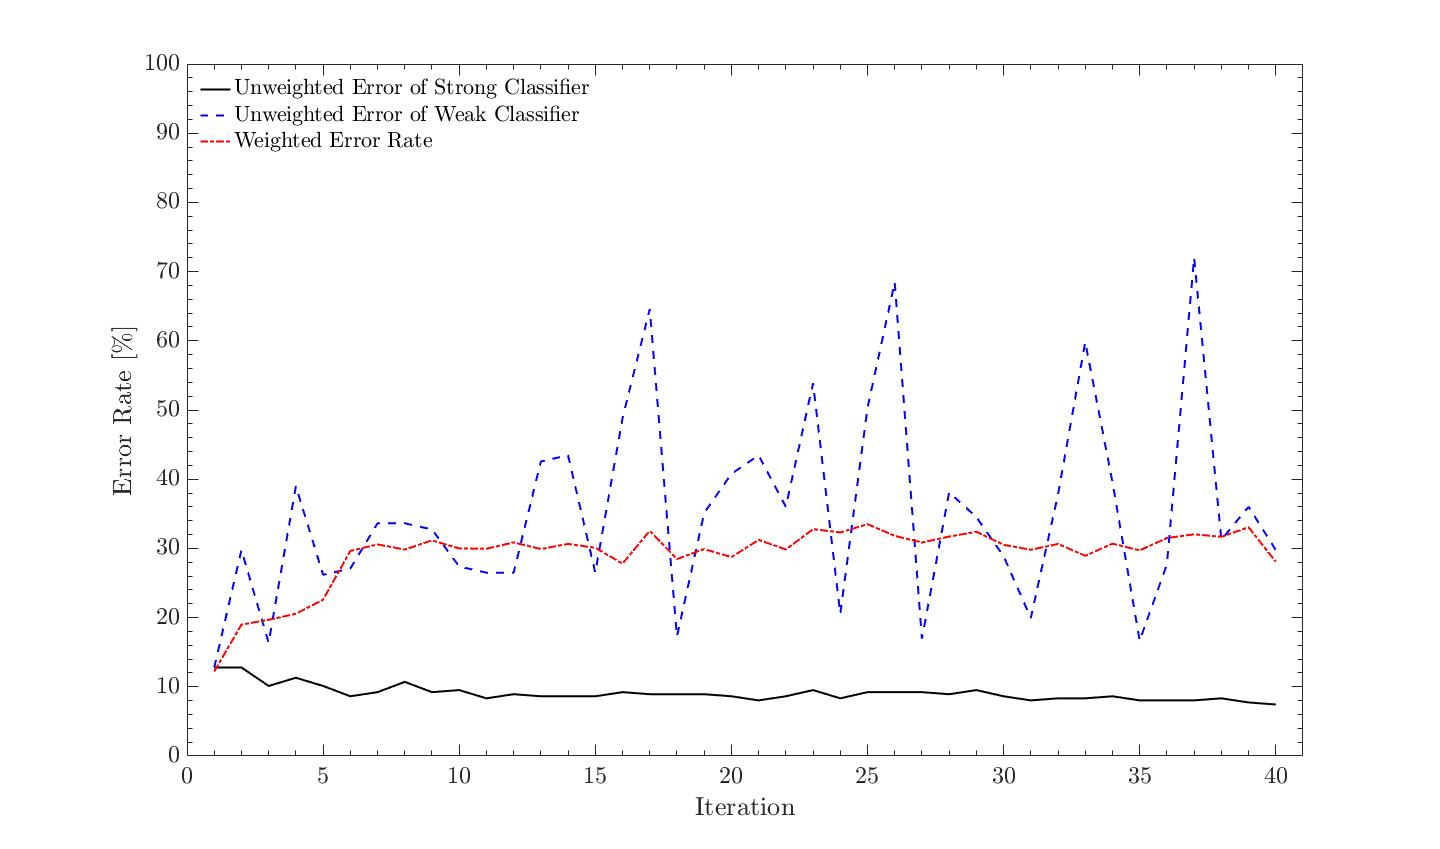
\includegraphics[width=\textwidth]{result}
		\caption{Facial Detection Errors Over 40 Iterations}
		\label{fig:result}
	\end{figure}
	
	\section{Discussion}
	\justify Over the 40 training iterations, the weighted error rate increases in the first 6 iterations and vacillates around 31 percent in later iterations. This is a result of the fact that we update the weight matrix $W$ after every iteration by reducing the weight of those correctly labeled features while raising that of the others. This also results in the non-convergence and the increasing error rate of the weak classifiers.\\
	\justify On the other hand, the strong classifier using Adaboost has a gradually decreasing error rate that converges to around 9 percent, an error rate much lower than that from any of the weak classifiers. Due to the way the weight matrix $W$ is updated, the weak classifier in the next iteration is designed to fix the mistake made by the current one. The alpha coefficients are designed to be larger for smaller error rate, and vice versa. So the whole strong classifier takes the advantage of all weak classifiers and output the best classification result.

\end{document}
